\PassOptionsToPackage{xetex}{xcolor}
\PassOptionsToPackage{xetex}{graphicx}
\documentclass[a4paper,landscape,headrule,footrule,xetex]{foils}

%%
%%%  Macros
%%%
\newcommand{\logo}{~}
\newcommand{\Story}{\SHA{FINA}{The Final Problem}}

\newcommand{\header}[3]{%
\title{\vspace*{-2ex} \Large DAS
\\\large  Semantics
\\[2ex] \Large  \emp{#2}}
\author{\blu{Francis Bond}   \\ 
  \normalsize  \textbf{Department of Asian Studies}\\
   \normalsize  \textbf{Palacký University}\\
\normalsize  \url{https://fcbond.github.io/}\\
\normalsize  \texttt{bond@ieee.org}}
\date{#1}
\renewcommand{\logo}{#2}
 \hypersetup{
   pdfinfo={
     Author={Francis Bond},
     Title={#1 #2},
     Subject={DAS Semantics},
     Keywords={Semantics, Pragmatics},
     License={CC BY 4.0}
   }
 %  pdfcopyright={Copyright © Francis Bond. Creative Commons 4.0 Attribution License.}
 %  pdflicenseurl={http://creativecommons.org/licenses/by/4.0/}
 }
}
%%
%% Multilingual Stuff
%%
\usepackage[a4paper,landscape,margin=25mm]{geometry}

\MyLogo{Semantics (2024); CC BY 4.0}



\usepackage{fontenc}
\usepackage{polyglossia}
\setmainlanguage{english}
\setmainfont{TeX Gyre Pagella}
\setsansfont[Ligatures=TeX]{TeX Gyre Heros}
\usepackage{xeCJK}
\setCJKmainfont{Noto Sans CJK SC}
\setCJKsansfont{Noto Sans CJK SC}
\setCJKmonofont{Noto Sans CJK SC}
%\setCJKttfont{Noto Sans CJK SC}
%\setCJKmainfont{WenQuanYi Micro Hei}
%\clearpage
%\setCJKmainfont{AR PL SungtiL GB}
\newfontfamily\ipafont{Charis SIL}
\newcommand\ipa[1]{\mtcitestyle{\ipafont #1}}


\usepackage[xetex]{xcolor}
\usepackage[xetex]{graphicx}
\newcommand{\blu}[1]{\textcolor{blue}{#1}}
\newcommand{\grn}[1]{\textcolor{green}{#1}}
\newcommand{\hide}[1]{\textcolor{white}{#1}}
\newcommand{\emp}[1]{\textcolor{red}{#1}}
\newcommand{\txx}[1]{\textbf{\textcolor{blue}{#1}}}
\newcommand{\lex}[1]{\textbf{\mtcitestyle{#1}}}

\usepackage{pifont}
\renewcommand{\labelitemi}{\textcolor{violet}{\ding{227}}}
\renewcommand{\labelitemii}{\textcolor{purple}{\ding{226}}}

\newcommand{\subhead}[1]{\noindent\textbf{#1}\\[5mm]}

\newcommand{\Bad}{\emp{\raisebox{0.15ex}{\ensuremath{\mathbf{\otimes}}}}}
\newcommand{\bad}{*}

\newcommand{\com}[1]{\hfill \textnormal{(\emp{#1})}}%
\newcommand{\cxm}[1]{\hfill \textnormal{(\txx{#1})}}%
\newcommand{\cmm}[1]{\hfill \textnormal{(#1)}}%
\usepackage{amssymb}
\usepackage{relsize,xspace}
\newcommand{\into}{\ensuremath{\rightarrow}\xspace}
\newcommand{\ent}{\ensuremath{\Rightarrow}\xspace}
\newcommand{\nent}{\ensuremath{\not\Rightarrow}\xspace}
\newcommand{\tot}{\ensuremath{\leftrightarrow}\xspace}
\usepackage{url}
\usepackage[hidelinks]{hyperref}
\hypersetup{
     colorlinks,
     linkcolor={blue!50!black},
     citecolor={red!50!black},
     urlcolor={blue!80!black}
}
%\usepackage{hyperxmp}
\newcommand{\lurl}[1]{\MyLogo{\url{#1}}}

\usepackage{mygb4e}
\let\eachwordone=\itshape
\newcommand{\lx}[1]{\textbf{\textit{#1}}}
\newcommand{\ix}{\ex\it}

\newcommand{\cen}[2]{\multicolumn{#1}{c}{#2}}
%\usepackage{times}
%\usepackage{nttfoilhead}
\newcommand{\myslide}[1]{%
\foilhead[-25mm]{\raisebox{12mm}[0mm]{\emp{#1}}}%
\leftheader{}%
\MyLogo{\logo}}

\newcommand{\mytask}[1]{%
\foilhead[-25mm]{\raisebox{12mm}[0mm]{\emp{#1}}}
\leftheader{🔍 Hi}%
\MyLogo{\logo}}

\newcommand{\myslider}[1]{\rotatefoilhead[-25mm]{\raisebox{12mm}[0mm]{\emp{#1}}}}
%\newcommand{\myslider}[1]{\rotatefoilhead{\raisebox{-8mm}{\emp{#1}}}}

\newcommand{\section}[1]{\myslide{}{\begin{center}\Huge \emp{#1}\end{center}}}

\usepackage{tcolorbox}
% \newcommand{\task}{\marginpar{\raisebox{-1ex}{\large
%       \tcbox[colframe=red,colback=white,arc=3pt]{\textbf{?}}}}}
% \newcommand{\task}{\marginpar{\raisebox{-1ex}{
%       \hspace{-0.5em}\tcbox[colframe=red,colback=white,arc=3pt]{%
%         \includegraphics[width=1.5em]{pics/detective}}}}}
\newcommand{\task}{\marginpar{\raisebox{-2ex}{
      \hspace{-0.5em}\reflectbox{\includegraphics[width=2em]{pics/detective}}}}}

\usepackage[lyons,j,e,k]{mtg2e}
\renewcommand{\mtcitestyle}[1]{\textcolor{teal}{\textsl{#1}}}
%\renewcommand{\mtcitestyle}[1]{\textsl{#1}}
\newcommand{\chn}{\mtciteform}
\newcommand{\cmn}{\mtciteform}
\newcommand{\cs}{\mtciteform}
\newcommand{\iz}[1]{\textup{\texttt{\textcolor{blue}{\textbf{#1}}}}}
\newcommand{\con}[1]{\textsc{#1}}
\newcommand{\gm}{\textsc}
\newcommand{\cmp}[1]{{[\textsc{#1}]}}
\newcommand{\sr}[1]{\ensuremath{\langle}#1\ensuremath{\rangle}}
\usepackage[normalem]{ulem}
\newcommand{\ul}{\uline}
\newcommand{\ull}{\uuline}
\newcommand{\wl}{\uwave}
\newcommand{\vs}{\ensuremath{\Leftrightarrow}~}
%%%
%%% Bibliography
%%%
\usepackage{natbib}
%\usepackage{url}
\usepackage{bibentry}


%%% From Tim
\newcommand{\WMngram}[1][]{$n$-gram#1\xspace}
\newcommand{\infers}{$\rightarrow$\xspace}



\usepackage{rtrees,qtree}
\renewcommand{\lf}[1]{\br{#1}{}}
\usepackage{avm}
%\avmoptions{topleft,center}
\newcommand{\ft}[1]{\textsc{#1}}
%\newcommand{\val}[1]{\textit{#1}}
\newcommand{\typ}[1]{\textit{#1}}
\avmfont{\sc}
%\avmvalfont{\sc}
\renewcommand{\avmtreefont}{\sc}
\avmsortfont{\it}


%%% From CSLI book
\newcommand{\mc}{\multicolumn}
\newcommand{\HD}{\textbf{H}\xspace}
\newcommand{\el}{\< \>}
\makeatother
\long\def\smalltree#1{\leavevmode{\def\\{\cr\noalign{\vskip12pt}}%
\def\mc##1##2{\multispan{##1}{\hfil##2\hfil}}%
\tabskip=1em%
\hbox{\vtop{\halign{&\hfil##\hfil\cr
#1\crcr}}}}}
\makeatletter

\newcommand{\sh}[1]{\lowercase{\href{https://fcbond.github.io/sh-canon/#1.html}}{#1}}
\newcommand{\SHA}[2]{\lowercase{\href{https://fcbond.github.io/sh-canon/#1.html}}{\textit{#2}}}

\newcommand{\zh}{\cmn}
\newcommand{\zsm}{\cmn}

\begin{document}
\header{Lecture 2}{Word meaning and close reading}{}
\maketitle

%\include{schedule}

\myslide{Overview}

\begin{itemize}
\item Word Meaning
  \begin{itemize}
  \item Definitions
  \item Translations/paraphrases
  \item Semantic Relations
  \item Components
  \item Derivational Relations
  \item Word Embeddings
  \end{itemize}
\item Wordnet
\item Close Reading and Word Sense Disambiguation
\end{itemize}

\section{The meanings of words}
 \MyLogo{}


\myslide{Words carry different meanings: \lex{leave}}
\MyLogo{\url{https://compling.upol.cz/ntumc/cgi-bin/showcorpus.cgi?sid_from=10000&sid_to=11000&clemma=leave}}
\begin{itemize} \addtolength{\itemsep}{0ex}
\item[10070] \eng{Nothing was \ul{left} save a few acres of ground , and the
  two-hundred-year-old house , which is itself crushed under a heavy
  mortgage .}
% leave (have left or have as a remainder) 
\item[10079] \eng{The money which my mother had \ul{left} was enough
  for all our wants , and there seemed to be no obstacle to our
  happiness . "}
%leave (leave or give by will after one's death;) 
\item[10085] \eng{He had no friends at all save the wandering
  gipsies , and he would give these vagabonds \ul{leave} to encamp upon
  the few acres of bramble- covered land which represent the family
  estate , and would accept in return the hospitality of their tents
  , wandering away with them sometimes for weeks on end .}
% leave (permission to do something;) 
\item[10107] \eng{She
  \ul{left} her room , therefore , and came into mine , where she sat for
  some time , chatting about her approaching wedding .}
%leave (move out of or depart from;) 
\item [10108]\eng{At
  eleven o'clock she rose to \ul{leave} me , but she paused at the door
  and looked back.}
%leave (move out of or depart from;) 
\item[10439] \eng{" The rest you will \ul{leave} in our hands
  . "}
% leave (put into the care or protection of someone;) 
\item[10449] \eng{And now , Miss Stoner , we must \ul{leave} you for if
  Dr. Roylott returned and saw us our journey would be in vain .
  }
% leave (move out of or depart from;) 
\item[10526] \eng{Then he turned down the lamp , and we were \ul{left} in darkness
  .}
% leave (act or be so as to become in a specified state;) 

\end{itemize}


How many different meanings?\task


\myslide{How can we represent the differences?}

\begin{itemize}
\item Definitions
\item Translations/paraphrases
\item Semantic Relations
\item Components
\item Derivational Relations
\item Word Embeddings
\end{itemize}


\myslide{Semantic Representations of Words}

\begin{itemize}\addtolength{\itemsep}{-1ex}
\item Divide meaning into
  \begin{itemize}
  \item \txx{reference}: the relation to the world/mental space
  \item \txx{sense}: the rest of the meaning
    \begin{itemize}
    \item \txx{denotation} the part that distinguishes the meaning
      from other meanings
    \item \txx{connotation}  cultural or emotional associations 
    \end{itemize}
  \end{itemize}
\item Introduce \con{concepts} %\hfill (meaning as font-change)
  \begin{itemize}
  \item How can we represent concepts?
  \item How do we learn them?
    \begin{itemize}
    \item Typically children start off by \txx{underextending} or \txx{overextending} concepts
    \end{itemize}
  \end{itemize}
\item Example: \eng{That dog}
  \begin{itemize}
  \item reference --- the animal over there
  \item sense --- canine quadruped domesticated by man
  \item connotation --- faithful, friendly (or dirty)
  \end{itemize}
\end{itemize}



\myslide{Definitional Semantics}

%\MyLogo{\citet{Jackson:2002,Wilks+:1996}}

\begin{itemize}
\item Standard lexicographic approach to lexical semantics:
  \begin{quote}
    \textbf{semantics} = \eng{the \textcolor{blue}{study} of \textcolor{brown}{language meaning}}\\
    \textbf{tailor} = \eng{a \textcolor{blue}{person} whose \textcolor{brown}{occupation is making and altering garments}}
  \end{quote}
\item Definitions are conventionally made up of;
  \begin{itemize}
  \item \textcolor{blue}{genus}: what class the lexical item belongs to
  \item \textcolor{brown}{differentiae}: what attributes distinguish it from
  other members of that class
\end{itemize}
% \item ``Decoding'' vs.\ ``encoding'' dictionaries
\item Often hard to understand if you don't already know the meaning!
\myslide{Definitional Semantics: pros and cons}
\item Pros:
  \begin{itemize}
  \item familiarity (we are taught to use dictionaries)
  \end{itemize}
\item Cons:
  \begin{itemize}
  \item subjectivity in sense granularity (splitters vs.\ lumpers) and
    definition specificity
  \item circularity in definitions
  \item consistency, reproducibility, \ldots
  \item often focus on diachronic (historical) rather than synchronic (current) semantics 
  \end{itemize}
\end{itemize}

\myslide{Entries for \lex{leave}}
\MyLogo{\url{https://compling.upol.cz/ntumc/cgi-bin/cgi-bin/wn-gridx.cgi?gridmode=ntumc-noedit&lang=eng&lemma=leave}}
\begin{description}
%  00613683-v (63)
% V2 	leave 	     	go and leave behind, either intentionally or by neglect or forgetfulness
\item [02015598-v] (72)
V1, V2 	\lex{get out, go out, leave, exit} ``move out of or depart from''
% 01494310-v (328)
% V2 	put, place, set, lay, position, pose, leave 	     	put into a certain place or abstract location
\item [02356230-v] (8)
V3 	\lex{leave, entrust} ``put into the care or protection of someone''
% 00053097-n (2)
% 	parting, farewell, leave, leave-taking 	     	the act of departing politely
      \item [02009433-v] (149)
V1 	\lex{leave, go away, go forth} ``go away from a place''
% 15139130-n (3)
% 	leave, leave of absence 	     	the period of time during which you are absent from work or duty
\item[02229055-v] (7)
V3 	\lex{leave, will, bequeath} ``leave or give by will after one's death''
% 02383440-v (14)
% V1, V2 	leave, depart, pull up stakes 	     	remove oneself from an association with or participation in
% 00360092-v (5)
% V2 	leave, leave behind 	     	be survived by after one's death
% 02721438-v (30)
% V2 	leave, allow for, allow, provide 	     	make a possibility or provide opportunity for; permit to be attainable or cause to remain
% 00136991-v (27)
% V2 	leave, leave alone, leave behind 	     	leave unchanged or undisturbed or refrain from taking
\item [02729414-v] (56) V2 	\lex{leave} ``act or be so as to become in a specified state''
\item [02730135-v] (5) V2 \lex{leave} ``have left or have as a remainder''

% 02635659-v (89)
% V2 	result, lead, leave 	     	have as a result or residue
% 02296153-v (27)
% V2, V3 	give, impart, leave, pass on 	     	transmit (knowledge or skills)
% 00613018-v (3)
% V2
\item [06690114-n] (1) \lex{leave} ``permission to do something''

\end{description}

Not to be confused with \eng{\ul{left} hand} and \eng{the \ul{leaves} fell}, \ldots .

\myslide{Paraphrases and translation}

\begin{itemize}
\item Saying the same thing in different words
  \begin{itemize}
  \item Same language = \txx{paraphrase}
  \item Different language = \txx{translation}
  \end{itemize}
\item We showed some paraphrases in the entries given above
\item If you speak another language, then you can use that to
  disambiguate may things.
  \begin{itemize}
  \item \lex{leave, entrust} = 預ける \jpn{azukeru}
  \item \lex{get out, go out, leave, exit} = 去る \jpn{saru}
  \item \lex{leave, will, bequeath} = 遺す \jpn{nokosu}
  \end{itemize}
\item Can you explain the ambiguity in \eng{The money which my mother
    had \ul{left} was enough for all our wants}?\task
\end{itemize}

% \myslide{Paraphrase cues}

% \begin{itemize}
% \item \lex{that is to say}
%   \begin{itemize}
%   \item  \eng{I met him that night, and he called next day to ask if we had got home all safe, and after that we met him - that is to say, Mr Holmes, I met him twice for walks, \ldots} IDEN
%   \item \eng{In three days, that is to say on Monday next  \ldots} FINA
%   \end{itemize}
% \item \lex{in other words}
%   \begin{itemize}
%   \item \eng{\ldots there is a possibility that these initials are those of the second person who was present - in other words, of the murderer. \ldots} BLAC
%   \item \eng{\ldots when they closed their League offices that was a sign that they cared no longer about Mr. Jabez Wilson's presence; in other words, that they had completed their tunnel.} REDH
%   \end{itemize}
% \end{itemize}


\myslide{Lexical Semantics}

\MyLogo{}

\begin{itemize}
\item Lexical semantics is concerned with the identification and
  representation of the semantics of lexical items
\item If we are to identify the semantics of lexical items, we have to
  be prepared for the eventuality of a given word having 
  multiple interpretations
  \begin{itemize}
  \item \txx{Polysemy}: having multiple meanings
  \item \txx{Monosemy}: having only one meaning
  \end{itemize}
\item \txx{Homonyms} are words with two unrelated meanings:
  \begin{itemize}
  \item \txx{homographs}: same spelling 
    \\ \eng{bow} vs \eng{bow}; \eng{keep} vs \eng{keep}
  \item \txx{homophones}: same pronunciation
     \\ \eng{right} vs \eng{write}; \eng{keep} vs \eng{keep}
  \end{itemize}

\end{itemize}






% \myslide{Polysemy}

% \MyLogo{\citet{Cruse:1986,Hirst:1987,_Ravin:Leacock:2000,Pustejovsky:1995}}

% \begin{itemize}
% \item \textbf{Polysemy} = the condition of a single lexical item having
%   multiple meanings
% \item Polysemy vs.\ homonymy (cf.\ \eng{bank} vs.\ \eng{bass})
% \item Polysemy vs.\ indeterminacy (cf.\ \eng{father} vs.\ \eng{uncle})
% \item Regular/logical vs.\ irregular polysemy (cf.\ \eng{ash})
% \item Regular vs.\ complementary polysemy (cf.\ \eng{door} vs.\ \eng{farm})
% \end{itemize}




\myslide{Distinguishing Polysemes}

%The polysemy of a word can be tested by a variety of means, including:
\begin{itemize}
\item \txx{Antagonism}: can the word be used in a sentence with
  multiple \underline{competing} interpretations that are incompatible? \\[1ex]
  \eng{Kim can't  bear children}
  \begin{itemize}
  \item Cannot have children
  \item Doesn't like children
  \end{itemize}
\item \txx{Zeugma}: can the word be used in a context where multiple
  \underline{competing} interpretations are simultaneously evoked? \\[1ex]
  \eng{Kim and her visa expired}
    \begin{itemize}
    \item died
    \item ran out
    \end{itemize}
 \eng{Hitmen were quite expensive, so she decided to take out a loan and her husband.} \task
  \item  \txx{Paraphrase/Translation}: Is there more than one (clearly different) way to paraphrase/translate the word.
  \end{itemize}

\myslide{Necessary and Sufficient Conditions}

\begin{itemize}
\item Can we define words in terms of \txx{conditions}?
  \begin{itemize}
  \item \lex{zebra}
    \begin{itemize}
    \item quadruped
    \item animal \com{redundant}
    \item black and white striped
    \item herbivore
    \end{itemize}
  \end{itemize}
\item These are \txx{intrinsic}, \txx{generic} properties
  ]
  \begin{itemize}
  \item An albino zebra with three legs is still a zebra
  \end{itemize}
\item Can we use words even if we don't know their properties?
  \begin{itemize}
  \item \lex{Kway Teow}
  \end{itemize}
\item We seem to be ok with fairly vague definitions
  \begin{itemize}
  \item What is a \lex{dog-cart}? \task
  \item What is a \lex{swamp adder}? \task
  \end{itemize}
\end{itemize}



\myslide{Words/Concepts are related in many ways}

We can also look at words (or more properly senses) in terms of their
relations to other words.

\begin{itemize}
\item \txx{Hyponymy/Hypernymy}
\item \txx{Synonymy}
\item \txx{Antonymy} (Opposites)
\item \txx{Meronymy}
    \begin{itemize}
    \item \txx{Member-Collection}
    \item \txx{Portion-Mass}
    \item \txx{Element-Substance}
    \end{itemize}
  \item \txx{Domain} (lexical field)
\end{itemize}





\myslide{Hypernymy and Hyponymy}

\begin{itemize}
\item \txx{Hyponymy}: X is a hyponym of Y iff
  $f(X)$ entails $f(Y)$ but $f(Y)$ does not entail $f(X)$ (for all or most $f$):
  \begin{quote}
    \eng{Kim has a pet \underline{dog} $\vDash$  Kim has a pet \underline{animal}}\\
    \eng{Kim has a pet \underline{animal} $\not\vDash$  Kim has a pet \underline{dog}}
  \end{quote}
  N.B.\ complications with universal quantifiers and negation:
  \begin{quote}
    \eng{Kim likes all \underline{animals} $\vDash$  Kim likes all \underline{dogs}}\\
    \eng{Kim likes all \underline{dogs} $\not\vDash$  Kim likes all \underline{animals}}
  \end{quote}
\item \txx{Hypernymy}: Y is a hypernym of X iff X is a hyponym of Y
\item Can a word have multiple hypernyms?
  \begin{exe}
    \ex \lex{tank$_1$} $\subset$ \lex{military\_vehicle$_1$}; $\subset$ \lex{tracked\_vehicle}$_1$; 
    $\subset$ \lex{armored\_vehicle$_1$}; ? $\subset$ \lex{weapon$_1$}
  \end{exe}
\end{itemize}


\myslide{What is \txx{entailment}}
\begin{quote}
  \txx{Entailment} ($\vDash$): A sentence $p$ entails a sentence $q$ when the
  truth of the first ($p$) guarantees the truth of the second ($q$),
  and the falsity of the second ($q$) guarantees the falsity of the
  first ($p$).
\end{quote}

\myslide{Properties of hypernymy/hyponymy}
  \begin{itemize}\addtolength{\itemsep}{-1ex}
  \item Asymmetric; applies at the sense level
  \item applies only to lexical items of the same word class
  \item Transitive: \lex{dog$_1$} $\subset$ \lex{mammal$_1$} $\subset$ \lex{animal$_1$}
  \item Not all nodes are lexicalized; can be multiple \\[2ex]
    \begin{tabular}{llll}
      neutral (Hyper) & male & female & child \\ \hline
%      pig & hog & sow & piglet\\
      \lex{sheep} & \lex{ram} & \lex{ewe} & \lex{lamb}\\
      \lex{cow} & \lex{bull} & \lex{\ul{cow}} & \lex{calf} \\
      \lex{goose} & \lex{gander} & \lex{\ul{goose}} & \lex{gosling}  \\
      \lex{horse} & \lex{stallion} & \lex{mare} & \lex{foal:colt/filly} \\
      \lex{dog} &  \lex{\ul{dog}} &  \lex{bitch} &\lex{puppy} \\
      \lex{snake} & \lex{\ul{snake}}& \lex{\ul{snake}}& \lex{\ul{snake}}\\
    \end{tabular}
  \item Can you do this for \lex{pig}, \lex{cat} or \lex{chicken}?\task
  \item Can you give an example of this in another language?\task
  \end{itemize}

\myslide{Language Change}

\begin{itemize}\addtolength{\itemsep}{-1ex}
\item The meanings of words change over time
\item \lex{guitar} --- ``a stringed instrument usually having six
  strings'': originally these all used the body to make sound
\item We then get \lex{electric guitar} --- ``a guitar with a built-in
  pickup or pickups which convert string vibrations into electrical
  signals for amplification''
\item To refer to non-electric guitars we get a new coining
  \lex{acoustic guitar} -- ``a guitar that does not require electrical
  amplification'': which used to just be guitar
  \begin{itemize}
  \item \lex{guitar} is now a hypernym of them both and can refer to
    either
  % \item we can also refer to the prototypical guitar (acoustic) using
  %   reduplication
  %   \\ \eng{What kind of guitar do you play?}  \eng{Guitar guitar}
  \end{itemize}
\newpage
  
\item Sometimes this practice becomes politically charged, although
  linguistically it is unremarkable
  \begin{itemize}
  \item \lex{woman} ``an adult female person''
  \item \lex{trans woman} ``a person who identifies as a woman but was assigned male at birth''
  \item \lex{cis woman}  ``a person who identifies as a woman and was assigned female at birth''
  \end{itemize}
  \item Can you give other examples of this in English or other languages?\task  
  
\end{itemize}
%mother, surrogate mother, stepmother, foster mother, god mother,
%adoptive mother, biological mother

% rice, cooked rice, chocolate rice, wild rice, brown rice
% 

\myslide{Synonymy}

\begin{itemize}
\item \txx{Propositional synonymy}: X is a propositional synonym of Y if
  \begin{itemize}
  \item   (i) X and Y are syntactically identical,
  \item (ii) substitution of Y  for X in a declarative sentence doesn't change its truth conditions
  \end{itemize}
  e.g., \lex{violin} and \lex{fiddle}
\item Why propositional synonymy is over-restrictive:
  \begin{itemize}
  \item syntactic identity (cf.\ \lex{eat} and \lex{devour})
  \item collocations (cf.\ \lex{cemetery} and \lex{graveyard})
  \item gradability (cf.\ \lex{sofa}/\lex{settee} vs.\ \lex{boundary/frontier})
  \end{itemize}
\end{itemize}

\myslide{Near Synonymy}
\begin{itemize}
\item Synonyms are substitutable in \textbf{some/most} rather than \textbf{all} contexts
\item Synonymy via semantics: synonyms share ``common traits'' or
  attributional overlap, walking the fine line between ``necessary
  resemblances'' and ``permissible differences'':
  \begin{quote}
      \lex{grain} vs. \lex{granule};  \lex{green} vs.\ \lex{purple}; \lex{alsation} vs. \lex{spaniel}
  \end{quote}
\item Permissible differentiation via \textbf{clarification}:
  \begin{quote}
    \eng{Here is a \underline{grain}, or \underline{granule}, of the substance.}\\
    \eng{* The cover is \underline{green}, \{or, that is to say\} \underline{purple}.}
  \end{quote}
  and \textbf{contrast}:
  \begin{quote}
    \eng{Here is a \underline{grain} or, more exactly, \underline{granule}}\\
    \eng{* He likes alsations, or more exactly, \underline{spaniels}}
  \end{quote}
\end{itemize}

\myslide{Properties of synonymy}

  \begin{itemize}
  \item Symmetric
  \item traditionally applies only to lexical items of the same word class
    \\ but pairs like \lex{can} vs \lex{be able to} suggest otherwise
  \item applied at the sense level?
  \item $\approx$ converse of polysemy
  \end{itemize}



\myslide{Antonymy (opposites)}

%\MyLogo{\citet{Cruse:1986,Miller:1990}}

\begin{itemize}
\item \txx{Simple antonyms}: the negative of one implies the positive of the other.
  \begin{exe}
    \ex \eng{dead/alive}
    \ex \eng{pass/fail}
  \end{exe}
\item \txx{Gradable Antonyms}: points  along a scale
  \begin{exe}
    \ex \eng{boiling/hot/warm/tepid/cool/cold/freezing}
    \ex \eng{like this class/fascinating/interesting/dull/boring}
  \end{exe}
\item \txx{Reverses}: reverse the direction of a motion
  \begin{exe}
    \ex \eng{ascend/descend}
    \ex \eng{up/down; right/left}
  \end{exe}
\newpage
\item \txx{Converses}: the same act from different points of view
  \begin{exe}
    \ex \eng{above/below; right/left}
    \ex \eng{employer/employee}
  \end{exe}
  (Slightly non-standard usage by Saeed)
\item \txx{Taxonomic Sisters}: children of the same (grand)parent
  \begin{exe}
    \ex \eng{Monday/Tuesday/\ldots{}/Sunday}
    \\ \textnormal{in WordNet:} \lex{day of the week} $\supset$ \lex{weekday}, \lex{weekend}
    \ex \eng{LMS/English/Chinese/\ldots}
    \\  \textnormal{Context dependent}
  \end{exe}
\end{itemize}

\myslide{Meronymy}

\begin{itemize}
\item \txx{Meronomy} refers to the part-whole relation
  \begin{itemize}
  \item \txx{meronym} is the part
  \item \txx{holonym} is the whole
  \end{itemize}
  \begin{tree}
    \br{\lex{car}}{
      \br{\lex{wheel}}{\lf{\lex{tire}} \lf{\lex{rim}}}
      \br{\lex{engine}}{\br{\lex{piston}}{} \br{\lex{valve}}{}}
      \br{\lex{door}}{}
      \br{\lex{steering wheel}}{}}
  \end{tree}
\item It is not always transitive
  \begin{tree}
      \br{\lex{shirt}}{
        \br{\lex{button}}{\br{\lex{button hole}}{}}}
   \end{tree} \\
  But we don't normally say that a \lex{button hole} is part of a \lex{shirt}.
\end{itemize}

\myslide{Member-Collection}

\begin{itemize}
\item The relation between a collection and one of the units that makes it up
  \begin{exe}
    \ex \eng{tree--forest}
    \ex \eng{sheep--flock}
    \ex \eng{fish--school}
    \ex \eng{book--library}
    \ex \eng{member--band}
    \ex \eng{musician--orchestra}
    \ex \eng{student--class}
  \end{exe}
\end{itemize}

\myslide{Portion-Mass}

\begin{itemize}
\item The relation between a mass noun and a typical unit of measurement
  \begin{exe}
    \ex \eng{drop--liquid}
    \ex \eng{grain--sand/salt/truth}
    \ex \eng{sheet/ream--paper}
    \ex \eng{lump--coal (or just about anything)}
    \ex \eng{strand--hair}
    \ex \eng{rasher--bacon}
  \end{exe}
\item Similar to classifiers in many ways, e.g. in Malay
  \begin{exe}
    \ex \eng[tail]{ekor}--\eng{animal}
    \ex \eng[human]{orang}--\eng{person}
  \end{exe}
\end{itemize}

\myslide{Domain (lexical field)}
\MyLogo{Examples from WordNet 3.0}
The domain in which a word is typically used with this meaning.

\begin{exe}
  \ex \lex{driver$_1$} --- the operator of a motor vehicle
  \ex \lex{driver$_2$} --- someone who drives animals that pull a vehicle
  \ex \lex{driver$_3$} --- a golfer who hits the golf ball with a driver [\con{golf}] 
  \ex \lex{driver$_4$} --- ($\simeq$ device driver) a program that determines how a computer will communicate with a peripheral device [\con{computer science}] 
  \ex \lex{driver$_5$} --- ($\simeq$ number one wood) a golf club (a wood) with a near vertical face that is used for hitting long shots from the tee [\con{golf}] 
\end{exe}

Some \con{golf} terms: \lex{approach$_9$}, \lex{approach shot$_1$}, \lex{golf course$_1$}, \lex{links course$_1$}, \lex{wedge$_5$}, \lex{tee$_1$}, \lex{scratch$_9$}, \lex{putt$_1$}, \lex{slice$_1$}, \lex{hook$_1$}

       % TOPIC TERM->(adj) dormie#1, dormy#1
       % TOPIC TERM->(adj) greenside#1
       % TOPIC TERM->(noun) approach#9, approach shot#1
       % TOPIC TERM->(noun) chip#8, chip shot#1
       % TOPIC TERM->(noun) driving iron#1, one iron#1
       % TOPIC TERM->(noun) golf-club head#1, club head#1, club-head#1, clubhead#1
       % TOPIC TERM->(noun) golf course#1, links course#1
       % TOPIC TERM->(noun) golf equipment#1
       % TOPIC TERM->(noun) golf range#1, driving range#1
       % TOPIC TERM->(noun) heel#6
       % TOPIC TERM->(noun) plus fours#1
       % TOPIC TERM->(noun) toe#4
       % TOPIC TERM->(noun) wedge#5
       % TOPIC TERM->(noun) whip#4
       % TOPIC TERM->(noun) loft#3
       % TOPIC TERM->(noun) address#7
       % TOPIC TERM->(noun) scratch#9
       % TOPIC TERM->(noun) card#8, scorecard#1
       % TOPIC TERM->(noun) apron#2
       % TOPIC TERM->(noun) divot#2
       % TOPIC TERM->(noun) divot#1
       % TOPIC TERM->(noun) greenskeeper#1
       % TOPIC TERM->(noun) medalist#2, medallist#2, medal winner#1
       % TOPIC TERM->(noun) stroke#6
       % TOPIC TERM->(noun) birdie#1
       % TOPIC TERM->(noun) bogey#2
       % TOPIC TERM->(noun) double-bogey#1
       % TOPIC TERM->(noun) eagle#2
       % TOPIC TERM->(noun) double eagle#1
       % TOPIC TERM->(noun) par#1
       % TOPIC TERM->(verb) address#10
       % TOPIC TERM->(verb) tee off#1
       % TOPIC TERM->(verb) par#1
       % TOPIC TERM->(verb) ace#3
       % TOPIC TERM->(verb) caddie#1, caddy#1
       % TOPIC TERM->(verb) eagle#2
       % TOPIC TERM->(verb) hole up#2
       % TOPIC TERM->(verb) carry#36
       % TOPIC TERM->(verb) toe#4
       % TOPIC TERM->(verb) shank#1
       % TOPIC TERM->(verb) putt#1
       % TOPIC TERM->(verb) putt#2
       % TOPIC TERM->(verb) heel#4
       % TOPIC TERM->(verb) toe#3
       % TOPIC TERM->(verb) drive#17
       % TOPIC TERM->(verb) hole#1, hole out#1
       % TOPIC TERM->(verb) slice#2
       % TOPIC TERM->(verb) hook#4
       % TOPIC TERM->(verb) sclaff#2
       % TOPIC TERM->(verb) sclaff#1
       % TOPIC TERM->(verb) tee#1, tee up#2
       % TOPIC TERM->(verb) chip#3
       % TOPIC TERM->(verb) birdie#1
       % TOPIC TERM->(verb) eagle#1, double birdie#1
       % TOPIC TERM->(verb) double bogey#1
       % TOPIC TERM->(verb) bogey#1


\myslide{And More}
\MyLogo{}
\begin{itemize}
\item There are many, many more lexical relations advocated by various
  theories including:
  \begin{itemize}
  \item Troponymy/hypernymy (cf.\ \eng{walk} vs.\ \eng{lollop}) 
    ``way of doing something''
  \item Entailment (cf.\ \eng{snore} vs.\ \eng{sleep}) ``if you do one thing, you must be doing the other''
  \item Operator (cf.\ \eng{question} vs.\ \eng{ask})
    ``the thing you do by doing something''
  \item Magnifier (cf.\ \eng{wound} vs. \eng{badly})
    ``intensifier, diminisher''
  \item Usage (cf.\ \eng{strong-willed} vs. \eng{pig-headed} ``stubborn'')
    \\ \eng{pig-headed} is \txx{pejorative}
%  \item[] $\vdots$
  \end{itemize}
\end{itemize}
% \section{Sentence Types}

\section{Componential Analysis}

\myslide{Break word meaning into its components}
\MyLogo{Inspired by work on phonetics in the Prague School}
\begin{itemize}
\item For example:
  \\[2ex] \begin{tabular}{lllll}
    \lex{woman} & \cmp{female} & \cmp{adult} & \cmp{human} & \\
    \lex{spinster} & \cmp{female} & \cmp{adult} & \cmp{human} & \cmp{unmarried} \\
    \lex{bachelor} & \cmp{male} & \cmp{adult} & \cmp{human} & \cmp{unmarried} \\
    \lex{wife} & \cmp{female} & \cmp{adult} & \cmp{human} & \cmp{married} \\
    \lex{girl} & \cmp{female} & \cmp{child} & \cmp{human} & \\
    \lex{boy} & \cmp{male} & \cmp{child} & \cmp{human} & \\
  \end{tabular}
  \\[2ex] \txx{semantic components}/\txx{primitives} shown as \cmp{component}
  \begin{itemize}
  \item components allow a compact description
  \item interact with morphology/syntax
  \item form part of our cognitive architecture
  \end{itemize}
\end{itemize}

\myslide{Defining Relations using Components}

\begin{itemize}
\item \txx{hyponymy}
  \begin{quote}
    A lexical item P is a hyponym of Q if all the components of Q are also in P.
  \end{quote}
  \begin{tabular}{lllll}
    \lex{woman} & \cmp{female} & \cmp{adult} & \cmp{human} & \\
    \lex{spinster} & \cmp{female} & \cmp{adult} & \cmp{human} & \cmp{unmarried} \\
%    \lex{bachelor} & \cmp{male} & \cmp{adult} & \cmp{human} & \cmp{unmarried} \\
    \lex{wife} & \cmp{female} & \cmp{adult} & \cmp{human} & \cmp{married} \\
  \end{tabular}
\\[2ex]  \lex{spinster} $\subset$ \lex{woman}; \lex{wife} $\subset$ \lex{woman}
\item \txx{incompatibility}
  \begin{quote}
    A lexical item P is incompatible with Q if they share some
    components but differ in one or more \txx{contrasting} components
  \end{quote}
%   \begin{tabular}{lllll}
% %    \lex{woman} & \cmp{female} & \cmp{adult} & \cmp{human} & \\
%     \lex{spinster} & \cmp{female} & \cmp{adult} & \cmp{human} & \cmp{unmarried} \\
% %    \lex{bachelor} & \cmp{male} & \cmp{adult} & \cmp{human} & \cmp{unmarried} \\
%     \lex{wife} & \cmp{female} & \cmp{adult} & \cmp{human} & \cmp{married} \\
%   \end{tabular}
  \lex{spinster} $\not\approx$ \lex{wife}

\end{itemize}

\myslide{Binary Features}

\begin{itemize}
\item We can make things more economical (fewer components):
  \\[2ex] \begin{tabular}{lllll}
    \lex{woman} & \cmp{+female} & \cmp{+adult} & \cmp{+human} & \\
    \lex{spinster} & \cmp{+female} & \cmp{+adult} & \cmp{+human} & \cmp{--married} \\
    \lex{bachelor} & \cmp{--female} & \cmp{+adult} & \cmp{+human} & \cmp{--married} \\
    \lex{wife} & \cmp{+female} & \cmp{+adult} & \cmp{+human} & \cmp{+married} \\
    \lex{girl} & \cmp{+female} & \cmp{-adult} & \cmp{+human} & \\
  \end{tabular}
  \begin{itemize}
  \item Which should be $+$? \cmp{+female} or \cmp{--male}
  \item Presumably also \cmp{--electric}, \cmp{--conical}, \ldots
    \\ Only show \txx{relevant} features
  \item \txx{antonyms} differ in only one binary component
  \end{itemize}
\end{itemize}

\myslide{Redundancy Rules}

\begin{itemize}
\item We can add relations between components:
\\[2ex]  \begin{tabular}{llll}
     \cmp{+human} & \into & \cmp{+animate}  \\
     \cmp{+adult} & \into & \cmp{+animate}  \\
     \cmp{+animate} & \into & \cmp{+concrete}  \\
     \cmp{+married} & \into & \cmp{+adult}  \\
     \cmp{+married} & \into & \cmp{+human}   & \ldots
  \end{tabular}
\item Which allows us to write:
  \\[2ex] \begin{tabular}{lllll}
    \lex{woman} & \cmp{+female} & \cmp{+adult} & \cmp{+human} & \\
    \lex{spinster} & \cmp{+female} & \cmp{+adult} & \cmp{+human} & \cmp{--married} \\
    \lex{bachelor} & \cmp{--female} & \cmp{+adult} & \cmp{+human} & \cmp{--married} \\
    \lex{wife} & \cmp{+female} & &   & \cmp{+married} 
  \end{tabular}
  \\[2ex] Can we say  \cmp{--married}  \into\  \cmp{+human}?
\end{itemize} 

\myslide{More Complex Breakdowns}

\begin{itemize}
\item We can add relations between components:
\\[2ex]  \begin{tabular}{llll}
     \cmp{+father} & \into & \cmp{+male} \cmp{+parent}  \\
     \cmp{+father}(\ul{x},y) & \into & \cmp{+male}(x) \cmp{+parent}(x,y) \\
     \cmp{+son}(\ul{x},y) & \into & \cmp{+male}(x) \cmp{+parent}(y,x) \\
     \cmp{+brother}(\ul{x},y) & \into & \cmp{+male}(x) 
     \cmp{+parent}(z,x) \cmp{+parent}(z,y) \\
     \cmp{+grandfather}(\ul{x},y) & \into & \cmp{+male}(x) 
     \cmp{+parent}(x,z)  \cmp{+parent}(z,y) \\
  \end{tabular}
\item Assume \cmp{+parent}(x,y)  means ``x is the parent of y''
\item There are various ways you can formalize such relationships
  \begin{itemize}
  \item Many parts of language can be formalized in such a way
  \item We did this for demonstratives
    \\ \lex{this, that, these, those, what, here, there, where}\task
  \end{itemize}
\end{itemize}


These are great for many sub-systems of language, but it is hard to make components for everything, \ldots

%%% FIXME inheritance

\myslide{Derivational Relations}

\begin{itemize}
\item There are also relations between meanings with different parts of speech
  \\ Here we say one word is derived from the other
\item Normally these have some morphological component
  \begin{itemize}
  \item \lex{beauty} (n) --- \lex{beautiful} (adj) --- \lex{beautifully} (adv) --- \lex{beautify} (verb)
  \item \lex{decision} (n) — \lex{decide} (v) — \lex{decisive} (adj) — \lex{decisively} (adv)
  \item \lex{drive} (v) — \lex{driver} (n) — \lex{drivable} (adj)
  \item \lex{creation} (n) — \lex{create} (v) — \lex{creative} (adj) — \lex{creatively} (adv)   \item \eng{Sandy \ul{cut} their hand} --- \eng{Sandy has a \ul{cut} on their hand}
  \end{itemize}
\end{itemize}

\myslide{Agentive Nouns}
\MyLogo{}
\begin{itemize}
\item An \txx{agentive noun} is a word that is typically derived from
  another word denoting an action, and that identifies an entity that
  does that action.  \\ \textbf{verb} + \lex{-er, -or, -ant}
  \begin{exe}
    \ex \lex{murderer, commentator, whaler, director, computer}
    \ex ?? \lex{undertaker, cooker, footballer} (Saeed also includes these)
  \end{exe}
\item Should \lex{murderer} be listed separately from \lex{murder} in
the dictionary? Why or why not?
\item Also \txx{recipient noun}s that show the undergoer:
  \textbf{verb} + \lex{-ee}: \lex{employee}, \lex{trustee}
\end{itemize}

\myslide{Agentive Nouns in Other Languages}
\MyLogo{Thanks to Yeo Jia Qi (Malay)}

\begin{itemize}
\item Japanese (suffix distinguishes person/machine)
  \begin{itemize}
  \item \zh{運転する} → \zh{運転者} \jpn[driver]{unten-sha}
  \item \zh{計算する} → \zh{計算者} \zh{計算機} \jpn[computer]{keisan-sha/ki}
  \item \zh{研究する} → \zh{研究者} \zh{研究員} \jpn[researcher]{kenkyuu-sha/in}
  \item \zh{読む} → \zh{読み手} \zh{読者} \jpn[reader]{yomite/dokusha}
  \end{itemize}
\item Malay (prefix can convert any part  of speech)
  \begin{itemize}
  \item \zsm[help]{bantu (v)} → \zsm[assistant/helper]{pembantu} 
  \item \zsm[cut]{potong (v)} → \zsm[cutter (human/machine)]{pemotong}
  \item \zsm[fly]{terbang (v)} → \zsm[pilot (not passenger)]{penerbang}
  %\item \zsm[scissors]{gunting (n)} → \zsm[(editor +human)]{penyunting}
  \end{itemize}

\end{itemize}



\myslide{Word Embeddings}
\MyLogo{Slides based on \href{https://www.shanelynn.ie/get-busy-with-word-embeddings-introduction/}{An introduction to word embeddings for text analysis} by Shane Lynn (2017)}


\begin{itemize}
\item Represent words as a vector of numbers (instead of a set of components)
\item Every word has a unique word embedding (or “vector”), which is
  just a list of numbers for each word.  
\item Embeddings start being useful from 50-500 dimensions
  \\ LLMs typically are much larger
\item The embedding captures the  “meaning” of the word. 
\item  Similar words end up with similar embedding values
\item Context based word embeddings give a different vector depending
  on the context 

\end{itemize}

\myslide{Word Embeddings}
\begin{itemize}
\item In the simplest case, each word is a number
\end{itemize}
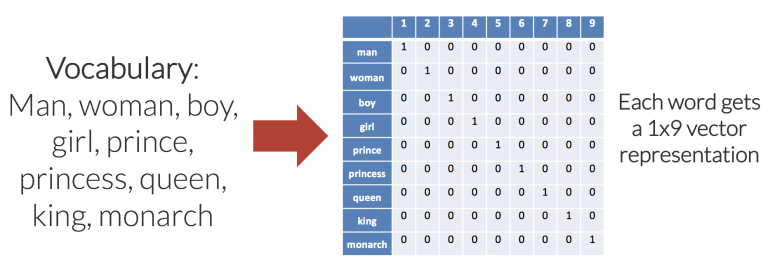
\includegraphics[width=\linewidth]{pics/one-hot-word-embedding-vectors-768x276.png}
\begin{itemize}\addtolength{\itemsep}{-2ex}
\item Two many dimensions
\item No shared information
\item Mainly zeros
\end{itemize}
\newpage
\begin{itemize}
\item We want fewer, more meaningful, dimensions (like components!) 
\end{itemize}
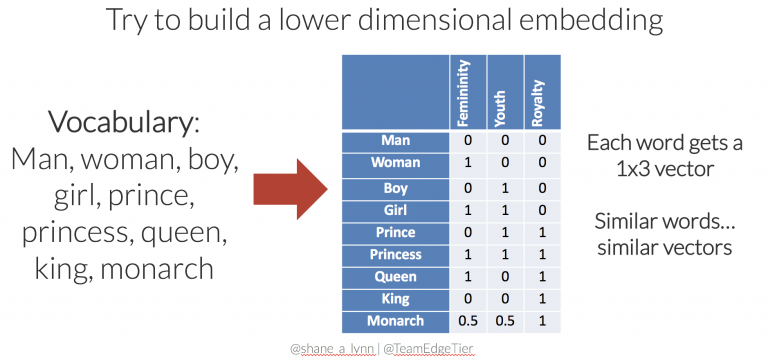
\includegraphics[width=\linewidth]{pics/3-dimensional-word-embeddings-example-768x362.png}

\begin{itemize}
\item How would you add \eng{child}? or \eng{emperor}?
\end{itemize}

\myslide{Similar words should be close}
\MyLogo{src: \url{http://suriyadeepan.github.io}}


\hspace{-4em}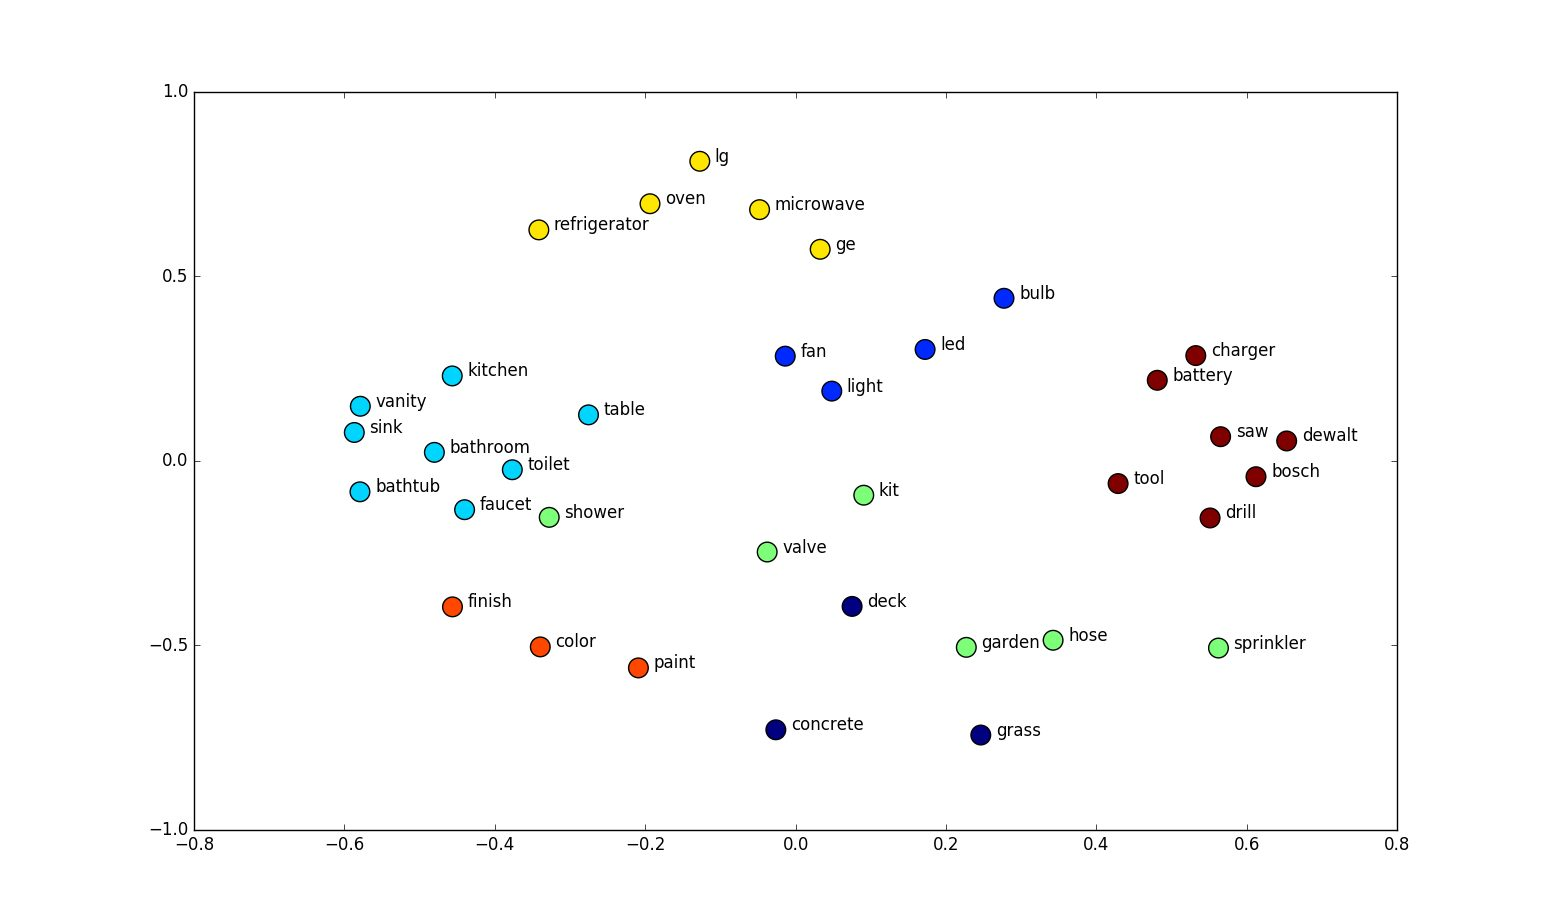
\includegraphics[width=1.1\linewidth]{pics/word-vector-space-similar-words.jpg}

\myslide{We can learn these from raw text}

\begin{itemize}
\item In LLMs, models are constructed to predict the context words from a
centre word, or the centre word from a set of context words.
\item By training on large amounts of text, embeddings that model human
intuitions can be built.
\item By using multilingual text, we can link languages
\item More about this in \textbf{DAS/LTI}: Language Technology and the Internet
\end{itemize}
\myslide{Semantic relations are also learned}


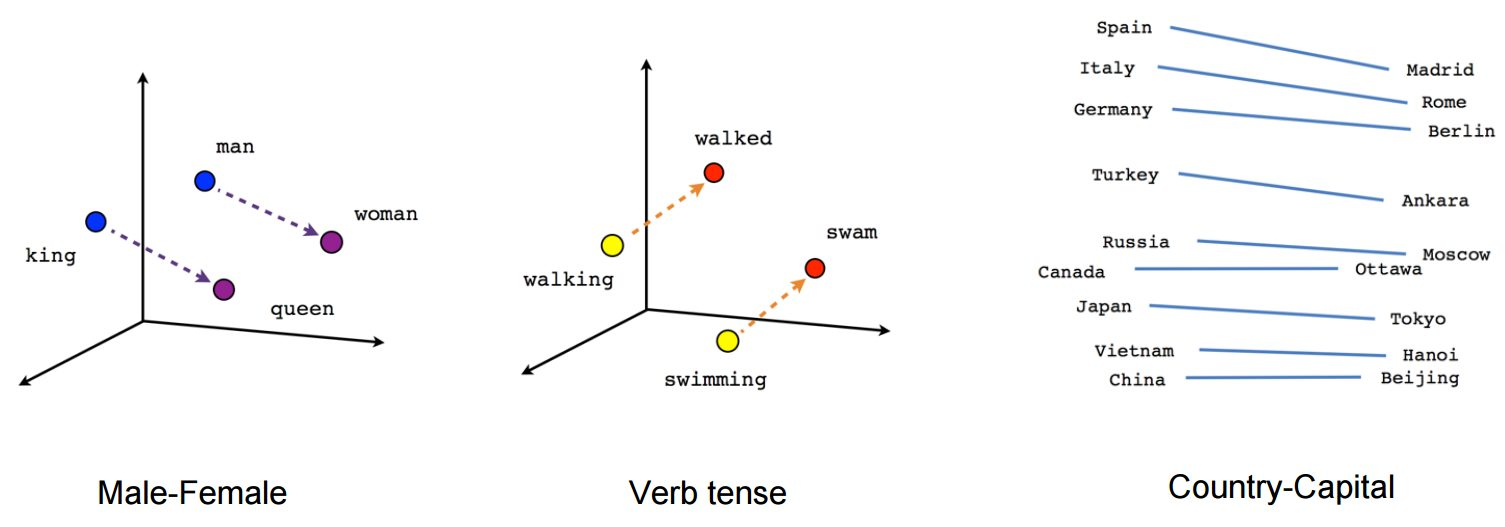
\includegraphics[width=\linewidth]{pics/vocabulary-linear-relationships.jpg}

We can do arithmetic on the vectors 


\begin{tabular}{rcl}
  $\vec{king}$ + $\vec{woman}$ $-$ $\vec{man}$  & $\approx$ & $\vec{queen}$ \\[2ex]
  $\vec{Paris}$ $-$ $\vec{France}$ + $\vec{Germany}$  & $\approx$ & $\vec{Berlin}$
\end{tabular}



\myslide{Corpora contain stereotypes, ML learns them!}

\begin{itemize}
\item We can test if things are closer to $\vec{he}$ or $\vec{she}$
  \\[2ex]
  \begin{tabular}{lcr}
    $\vec{nurse}.\vec{she}$ & = & 0.38 \\
    $\vec{nurse}.\vec{he}$ & = & $-0.12$ \\
    $\vec{programmer}.\vec{she}$ & = & 0.07 \\
    $\vec{programmer}.\vec{he}$ & = & 0.28 \\
  \end{tabular}
\end{itemize}

\begin{itemize}
\item This is an accurate description of the state of the world described in the corpus
\item But may not be what we want to use as a basis for reasoning, \ldots
\end{itemize}

\MyLogo{\citet{10.5555/3157382.3157584}}


\section{Wordnet}
\MyLogo{A graph-based approach}

\myslide{WordNet}

\MyLogo{\citet{Miller:1998:foreword,_Fellbaum:1998}}

\begin{itemize}
\item WordNet is an open-source electronic lexical database of English,
  developed at Princeton University
  \begin{quote}
    \url{http://wordnet.princeton.edu/}
  \end{quote}
\item Made up of four separate semantic nets, for each of nouns, verbs,
  adjectives and adverbs
\item WordNets exist for many languages, my group has worked on:
  \begin{itemize}
  \item Japanese 
  \item Bahasa Malay/Indonesian
  \item Chinese (Mandarin and Cantonese)
  \item The shared open multi-lingual wordnet (150+ languages) 
    \\ \url{https://omwn.org/}
  \item Kristang
  \item Myanmar
  \item Czech
\end{itemize}
\end{itemize}

\myslide{Wordnet Structure}
\begin{itemize}
\item Lexical items are categorised into $\sim$115K (and counting) glossed \textbf{synsets} (= synonym sets)

  \begin{quote}\smaller[2]
\begin{verbatim}
1. enrichment -- (act of making fuller or more 
   meaningful or rewarding)
2. enrichment -- (a gift that significantly increases 
   the recipient's wealth)
\end{verbatim}
  \end{quote}
\item Lexical relations at either the synset level or sense (=
  combination of lexical item and synset) level 
\item Strongly lexicalist (orginally):
  \begin{itemize}
  \item synsets only where words exist
  \item but many multiword expressions ($\approx 50\%$)
%  \item (near) absence of frame semantics
  \end{itemize}

% \newpage

% \item Other quirks/properties:
%   \begin{itemize}
%   \item 25 \textbf{unique beginners} in noun semantic net
%   \item taxonomic vs.\ functional hyponymy (cf.\ \eng{chicken} vs.\
%     \eng{bird/food})
%   \item few proper nouns and no separate classification for proper nouns
%   \end{itemize}
\end{itemize}





\myslide{Psycholinguistic Foundations of WordNet}

\MyLogo{}

\begin{itemize}
\item Strong foundation on hypo/hypernymy (lexical inheritance) based on
  \begin{itemize}
  \item   response times to sentences such as:
    \begin{quote}%\smaller
      \eng{a canary \{can sing/fly,has skin\}}\\
      \eng{a bird \{can sing/fly,has skin\}}\\
      \eng{an animal \{can sing/fly,has skin\}}
    \end{quote}
  \item analysis of anaphora:
    \begin{quote}%\smaller
      \eng{I gave Kim a novel but the \{book,?product,...\}
        bored her}\\
      \eng{Kim got a new car. It has shiny \{wheels,?wheel nuts,...\}}
    \end{quote}
  \item selectional restrictions
  \end{itemize}
\item Is now often used to calculate \txx{semantic similarity}
  \begin{itemize}
  \item The shorter the path between two synsets the more similar they are
  \item Or the shorter the path to the nearest shared hypernym, \ldots
  \end{itemize}
\end{itemize}


\myslide{Word Meaning as a Graph}
\MyLogo{}
\bigskip
\bigskip
\bigskip
\includegraphics[height=0.75\textheight]{pics/Semantic_Net.eps}

\begin{itemize}
\item You need a very big graph to capture all meanings
\end{itemize}



\myslide{Wordnet in this course}


\begin{itemize}
\item We will use wordnet to test our skills in determining word meaning
  \begin{itemize}
  \item tag a short text from this year's story or stories
  \item discuss differences with other annotators
 \end{itemize}
\item As well as a source of examples and inspiration
\end{itemize}
\section{Word Sense Disambiguation \\ for Close Reading}



\myslide{Close Reading}
\MyLogo{The idea comes from the study of poetry and is part of the
  school of \textit{New Criticism}  \citep[e.g.,][]{Brooks:Warre:1938,Brooks:Warre:1943}}

\begin{itemize}
\item Reading (and often re-reading) a text to uncover multiple
  aspects of meaning that lead you to understand a text better
\item Looking at what the text actually says, as well as the
  inferences you make from reading it
\item After a close reading you should be able to support your
  conclusions with specific examples from the text
\item You can consider many aspects of the text, such as
  \begin{itemize}
  \item The Title
  \item Word Choice
  \item The Tone and Style
  \item Discerning Patterns
    % Does an image here remind you of an image elsewhere in the book? Where? What's the connection?
    % How might this image fit into the pattern of the book as a whole?
    % Could this passage symbolize the entire work? Could this passage serve as a microcosm--a little picture--of what's taking place in the whole work?
    % What is the sentence rhythm like? Short and choppy? Long and flowing? Does it build on itself or stay at an even pace? What is the style like?
    % Look at the punctuation. Is there anything unusual about it?
    % Is there any repetition within the passage? What is the effect of that repetition?
    % How many types of writing are in the passage? (For example, narration, description, argument, dialogue, rhymed or alliterative poetry, etc.)
    % Can you identify paradoxes in the author's thought or subject?
    % What is left out or kept silent? What would you expect the author to talk about that the author avoided?
  \item  Point of View and Characterization
  \item Symbolism

    % How does the passage make us react or think about any characters or events within the narrative?
    % Are there colors, sounds, physical description that appeals to the senses? Does this imagery form a pattern? Why might the author have chosen that color, sound or physical description?
    % Who speaks in the passage? To whom does he or she speak? Does the narrator have a limited or partial point of view? Or does the narrator appear to be omniscient, and he knows things the characters couldn't possibly know? (For example, omniscient narrators might mention future historical events, events taking place "off stage," the thoughts and feelings of multiple characters, and so on).
  \end{itemize}
  \end{itemize}

\myslide{Word Choice and Diction}
\MyLogo{We will focus on this}

\begin{itemize}
\item What word(s) stand out? Why? (typically vivid words, unusual choices, or a contrast to what a reader expects)
\item How do particular words get us to look at characters or events in a particular way? Do they evoke an emotion?
\item Did the author use nonstandard language or words in another language? Why? What is the effect?
\item Are there any words that could have more than one meaning? Why might the author have played with language in this way?
\item Do some words have extra connotations?
\end{itemize}

\myslide{Word Sense Disambiguation}

\begin{itemize}
\item Knowing what individual words mean is the first step towards understanding
\item We will try to identify the \txx{sense} of words
  \begin{itemize}
  \item We use \href{https://wordnet.princeton.edu/}{Wordnet} \citep{_Fellbaum:1998} as the sense inventory
    \\ because it contains semantic relations as well as definitions
    \\ and it is accessible: there are good interfaces to it
  \item For every word we chose the most appropriate sense in wordnet
    \\ or write a comment if we think there isn't one
  \item Once we have identified a sense, it is then easy to look at
    synonyms and other closely related words
  \item We use the Czech wordnet \citep{Pala:Smrz:2004} for Czech
  \item Both wordnets have been extended as part of the the Natural Text Understanding --- Multilingual Corpus (\txx{ntu-mc})
  \end{itemize}
  \newpage
\myslide{WSD: Example}

 \eng{Sherlock Holmes had been leaning back in his chair with his
    eyes closed and his head sunk in a cushion, but he half opened his
    \ul{lids} now and glanced across at his visitor.}\task{}
  \begin{enumerate}\small
  \item \lex{hat, chapeau, lid} ``headdress that protects the head
    from bad weather; has shaped crown and usually a brim''
  \item \lex{lid, eyelid, palpebra} ``either of two folds of skin that
    can be moved to cover or open the eye''
  \item \lex{lid} ``a movable top or cover (hinged or separate) for closing the opening at the top of a box, chest, jar, pan, etc.''  \end{enumerate}
 
 \newpage
\myslide{WSD: A challenging task!}
This is difficult for many reasons
  \begin{itemize}
  \item Meaning boundaries are not clear: the sense distinctions
    impose a structure on something that is actually fuzzy
  \item Dictionaries are imperfect
    \begin{itemize}
    \item senses may be missing
    \item senses may be too fine-grained
    \end{itemize}
  \item Processing a text by computer is difficult
    \begin{itemize}
    \item The computer may have misinterpreted
    \begin{itemize}
    \item the part-of-speech
      \\ \eng{Does that go}  ``Female deer which go'' ``Is it the case that is goes?''
      \\ \eng{The speckled band} ``the band that is speckled'' ``the band that someone speckled''
    \item Or the sentence boundaries
    \item Or the words boundaries
    \end{itemize}
        \end{itemize}
  \item People use language idiosyncratically 
    \begin{itemize}
    \item extending meanings metaphorically
    \item sometimes so strangely that we might even say wrongly
    \end{itemize}
  \end{itemize}
  \myslide{WSD:  not impossible}
    \begin{itemize}
  \item Typically people agree around 72.5\% of the time \citep{Snyder:Palmer:2004}.
    \begin{itemize}
    \item  Verbs are hardest (67.8\%), then nouns (74.9\%) and adjectives (78.5\%)
    \item Disagreements tend to cluster around a relatively small group of difficult words.
    \item For example \lex{national}
      \begin{itemize}
      \item In six out of seven instances one annotator chose
        ``limited to or in the interests of a particular nation'' and
        the other annotator chose ``concerned with or applicable to or
        belonging to an entire nation or country''
      \item They are hard to distinguish!
      \end{itemize}
    \end{itemize}
  \end{itemize}
\end{itemize}

\myslide{Projects 1 and 2}
\MyLogo{Details online: we will give a demo}
\begin{itemize}
\item[1] Identify and annotate word meaning for your own passage of
  one of the stories using wordnet as the sense inventory: 3 or 4 people do
  the same set of sentences.
  \begin{itemize}
  \item For every word that needs to be tagged, either
    \begin{itemize}
    \item Chose a sense in wordnet
    \item Identify it as a named entity
    \item Identify a problem in the corpus or wordnet
      \\ and leave a comment saying what the it should be
    \end{itemize}
  \item Do this on your own --- the goal is to think about the words' meanings
  \end{itemize}
\item[2] Compare and contrast your annotations with other annotators;
  re-annotate based on your discussion and leave comments for at least
  five words.
  \begin{itemize}
  \item We expect you to disagree 30-40\% of the time (more often than experts)
  \item Sometimes you will have made a careless mistake
  \item Sometimes you will have interpreted wordnet differently
  \item Sometimes you will have interpreted the passage differently
  \item Discussing meaning deepens your understanding of it
  \end{itemize}
\end{itemize}








\myslide{Conclusions}

\begin{itemize}
\item We learned a little about word meaning, wordnet, close reading and your assignment
\item This is covered in more detail in \citet[Chapter 3]{Saeed:2015}
\end{itemize}


\myslide{Acknowledgments and References}

\begin{itemize}
\item Definitions from WordNet: \url{http://wordnet.princeton.edu/}
\item Images from
  \begin{itemize}
  \item the Open Clip Art Library: \url{http://openclipart.org/}
  \item Steven Bird, Ewan Klein, and Edward Loper (2009) 
     \textit{Natural Language Processing with Python}, O'Reilly Media
    \\ \url{www.nltk.org/book}
\end{itemize}
%\item Problems  partially based on exercises from Saeed (2003)
\item Video: Dead parrot sketch by Monty Python
\end{itemize}









  
\small
\bibliographystyle{aclnat}
\bibliography{abb,mtg,nlp,ling}





\end{document}

%%% Local Variables: 
%%% coding: utf-8
%%% mode: latex
%%% TeX-PDF-mode: t
%%% TeX-engine: xetex
%%% End: 

